\section{L1 computation}

\begin{frame}{L1 Eventbuilding}{}
	\begin{block}{L1 Eventbuilding}
		L1 trigger executed not before all L0 data has been received \\
		$\Rightarrow$ L1 algorithms have access to full event (except LKr data)
	\end{block}
	
	\begin{exampleblock}{All detectors processed within one thread}
		You can define the (most efficient) order of the algorithms\\
		e.g. execute most CPU demanding parts at last
	\end{exampleblock}
\end{frame}

\begin{frame}[fragile]
\frametitle{L1 interface}
After successfully collecting all L0 data of one event the following method is
invoked:
\begin{lstlisting}[frame=trBL,caption={}]{}
const uint16_t L1TriggerProcessor::compute(Event* event) {
    // Your code comes here
    ...
    return (L0Trigger + L1Trigger<<8);
}
\end{lstlisting}
if L1Trigger==0 the event will be discarded by the framework
\end{frame}


\begin{frame}{Event data structure}{}
\begin{center}
  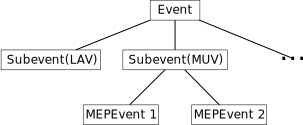
\includegraphics[width=6cm]{event-data-structure}
\end{center}
MEPEvent: The actual raw data struct as received via a MEP. Each
subevent has as many MEPEvents as sources (Tel62 boards) are sending MEPs.
\end{frame}

\begin{frame}[fragile]
\frametitle{Accessing the raw data}
Event has one getter function for each detector:
\begin{lstlisting}[frame=trBL,caption={}]{}
Subevent* muv=event->getMUVSubevent();
for (int p = muv->getNumberOfParts()-1;  p >= 0; p--) {
  MEPEvent* mepData = muv->getPart(p);
  mepData->getSourceID();
  mepData->getData();
  mepData->getEventLength();
}
\end{lstlisting}
\end{frame}

\begin{frame}[fragile]
\frametitle{L0TP}
Some data has to be taken from the L0TP data:
\begin{lstlisting}[frame=trBL,caption={}]{}
MEPEvent* L0TPEvent = event->getL0TPSubevent()->getPart(0);

//Struct L0TP has to be defined:
L0TP* L0TPData = (L0TP*) L0TPEvent->getData();
event->setFinetime(L0TPData->fineTime);
\end{lstlisting}
\end{frame}

\section{L2 computation}
\begin{frame}[fragile]
\frametitle{L2interface}
After successfully collecting all CREAM data of one event the following method
is invoked with the very same Event object:
\begin{lstlisting}[frame=trBL,caption={}]{}
const uint8_t L2TriggerProcessor::compute(Event* event) {
    // Your code comes here
    ...
    return L2Trigger;
}
\end{lstlisting}
Event may be used for L1$\rightarrow$L2 communications
\end{frame}

% \begin{frame}[fragile]
% \frametitle{CREAM data}
% Accessing the CREAM data has to be done by crateID and CREAMID:
% \begin{lstlisting}[frame=trBL,caption={}]{}
% LKREvent* lkrEvent = event->getLKrEvent(crateID, creamID);
% lkrEvent->getData();
% lkrEvent->getEventLength();
% \end{lstlisting}
% \end{frame}

\section{Constraints}
\begin{frame}{Constraints for the trigger implementations}{}
There are no constraints concerning CPU time or memory consumption:
The more you need, the more PCs you have to buy!

\begin{itemize}
  \item Do not use any kind of parallelisation without asking me!!!
  \item Do not free any memory coming from *event
  \item Use Eclipse for development: (code completion, easy debugging, auto
  make, refactoring\ldots)
\end{itemize}
\end{frame}

\section{Future approach}
\begin{frame}{Accessing the code}{}
The code (eclipse project) is available under CERN SVN:\\ \\
svn co https://svn.cern.ch/reps/na62-farm/na62-farm \\

Access has to be requested via mail: kunzej@cern.ch

\begin{block}{Dependencies/Prerequisites}
\begin{enumerate}
  \item boost and tcmalloc (run install/install.sh)
  \item Root access
  \item PCIe network device
  \item pf\_ring: (installed via install/install.sh)
\end{enumerate}

I can implement a low performance version to get rid of points 2-4

\end{block}
\end{frame}

\begin{frame}{To be done}{}
\begin{block}{Simulation with MC data}
 Only simple Tel62/CREAM simulators exist sending random data
\end{block}
\begin{ergo}
If someone generates MEP files out of MC data I can implement the transmitter
needed to test the L1/L2 algorithms
\end{ergo}
\end{frame}

\section{Summary}
\begin{frame}{Summary}{}
\begin{itemize}
  \item You can put your algorithms into na62-farm/l[12]
  \item Someone has to manage L[12]TriggerProcessor::compute (order of
  algorithms)
  \item Someone has to provide me MC data in the MEP format
  \item Please request access to the repository the next 10 days!
  \item Feel free to: ssh root@na62farm6 "eclipse"
\end{itemize}
\end{frame}